Most drawings have not been updated from the Concepts Report. These will be modified for the Design Dossier.
Ultimately, the modifications are purely internal and will not influence the external kinematic analysis. The only major change was the distribution of components within the chassis, in order to calculate a more adequate centre of mass. The arrangement in Figure \ref{fig:crab_top_view} is thus replaced by the arrangement shown further on in Figure \ref{fig:component_layout}. 

\begin{figure}
    \centering
    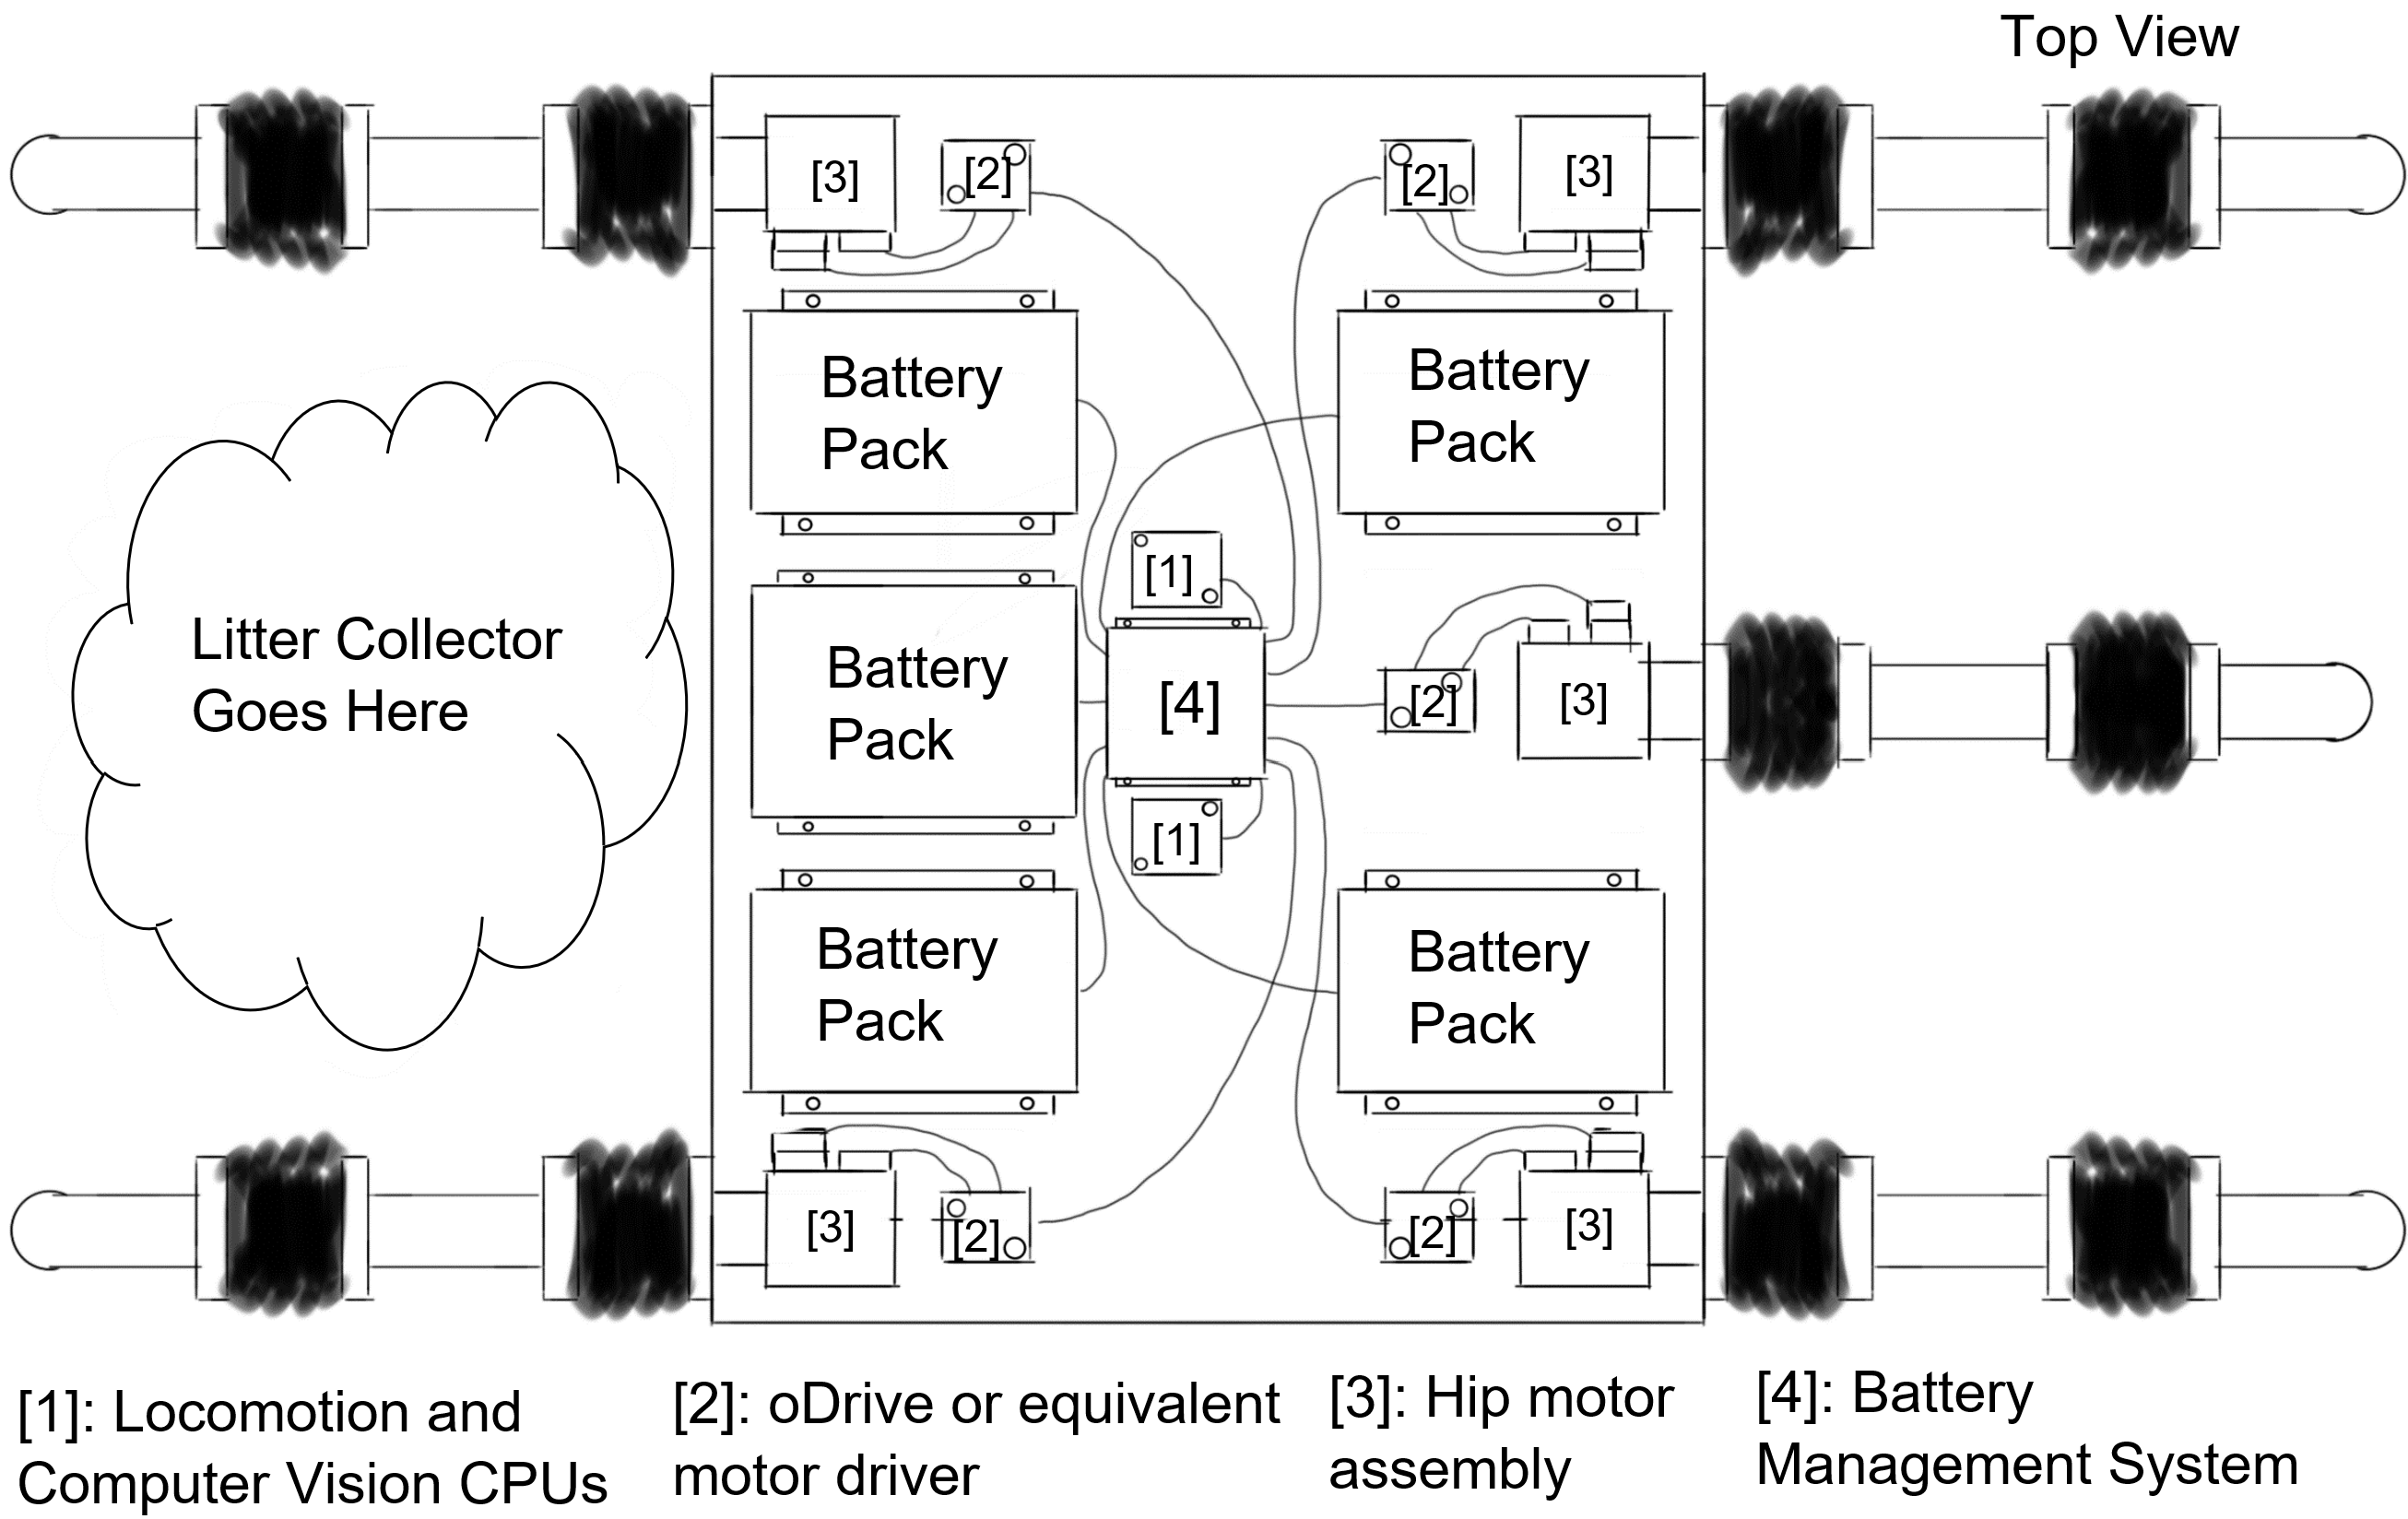
\includegraphics[width=0.9\textwidth]{2_DesignSolution/img/crab_top_view.png}
    \caption{Crab Top View}
    \label{fig:crab_top_view}
\end{figure}

\begin{figure}
    \centering
    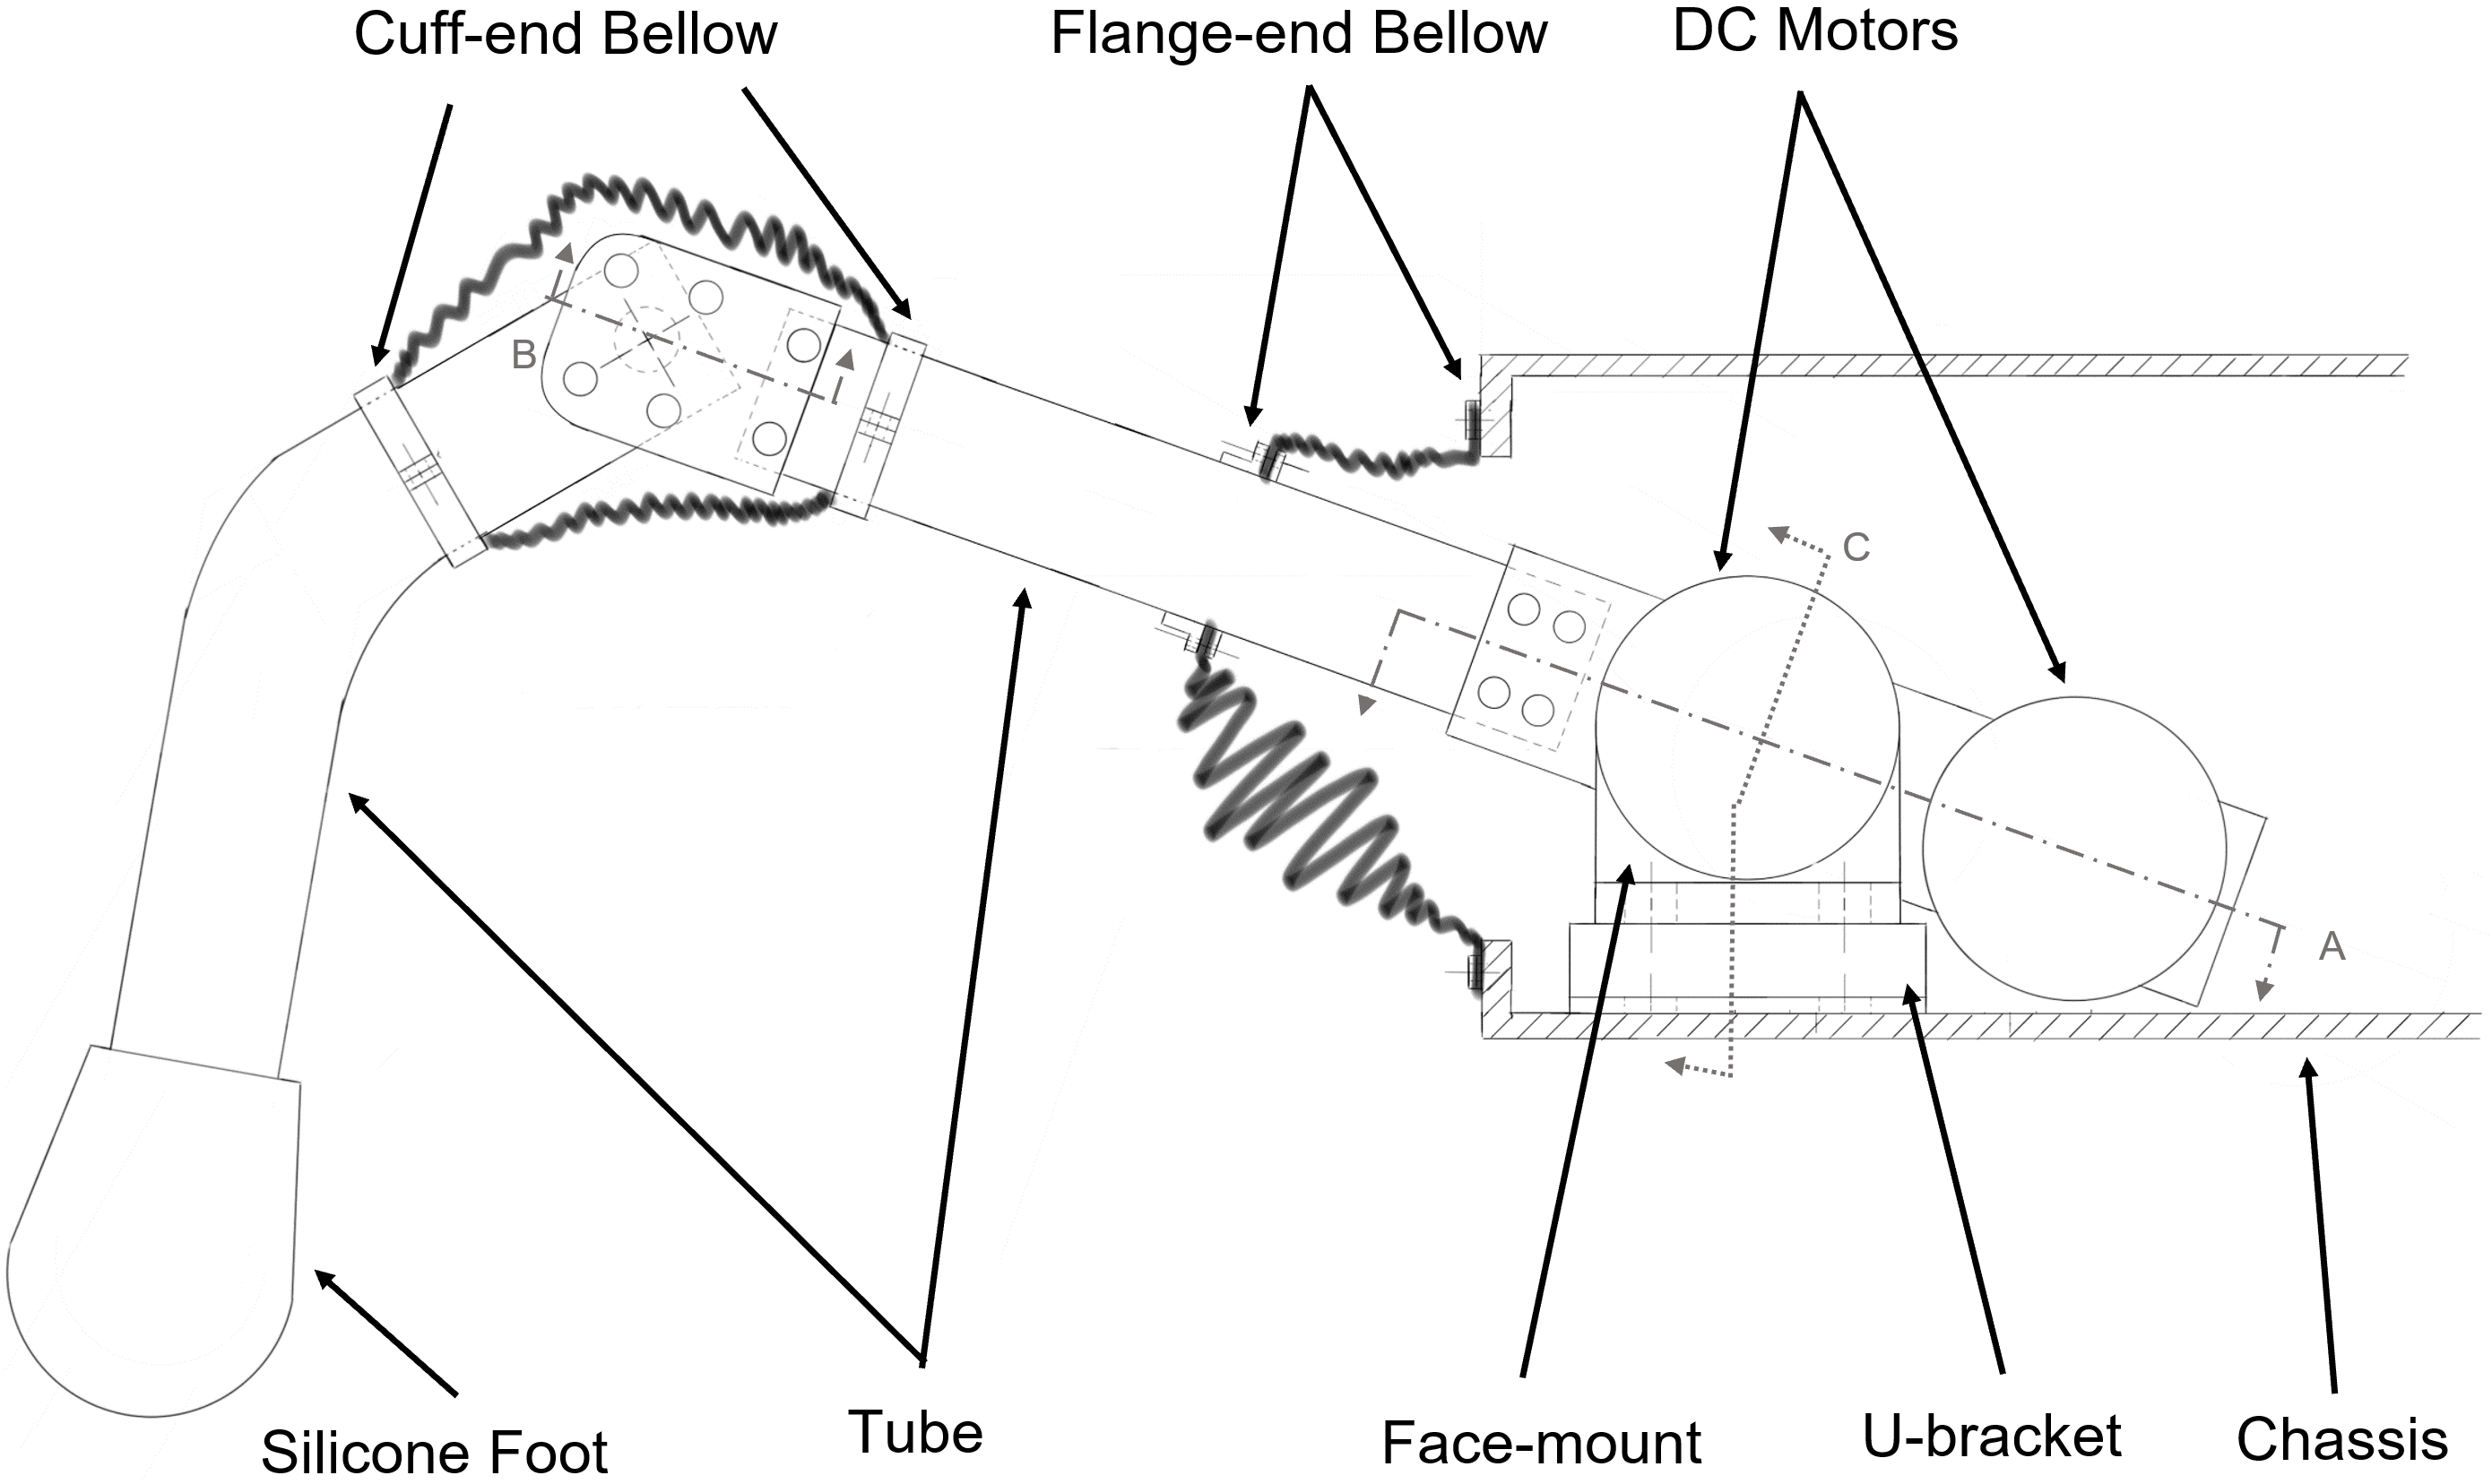
\includegraphics[width=0.8\textwidth]{2_DesignSolution/img/crab_leg.png}
    \caption{Crab Leg Side View}
    \label{fig:crab_leg}
\end{figure}

\begin{figure}
    \centering
    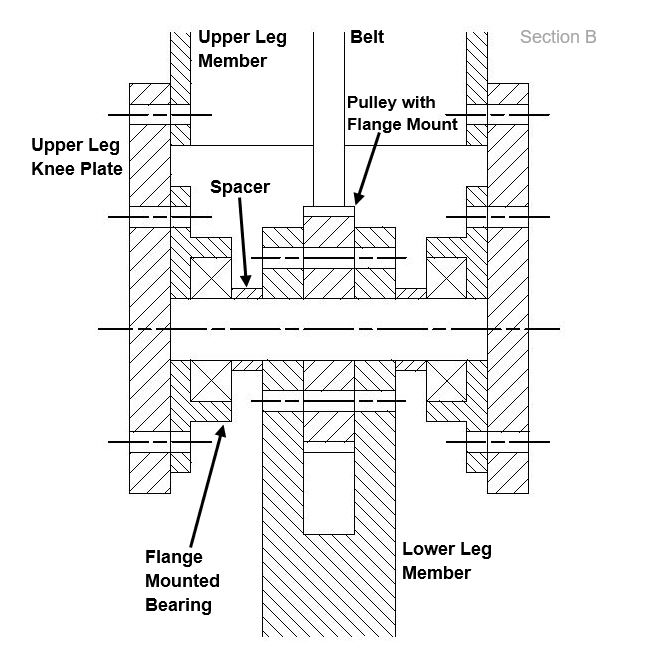
\includegraphics[width=0.7\textwidth]{2_DesignSolution/img/crab_knee.JPG}
    \caption{Crab Knee Top View}
    \label{fig:crab_knee}
\end{figure}

\begin{figure}
    \centering
    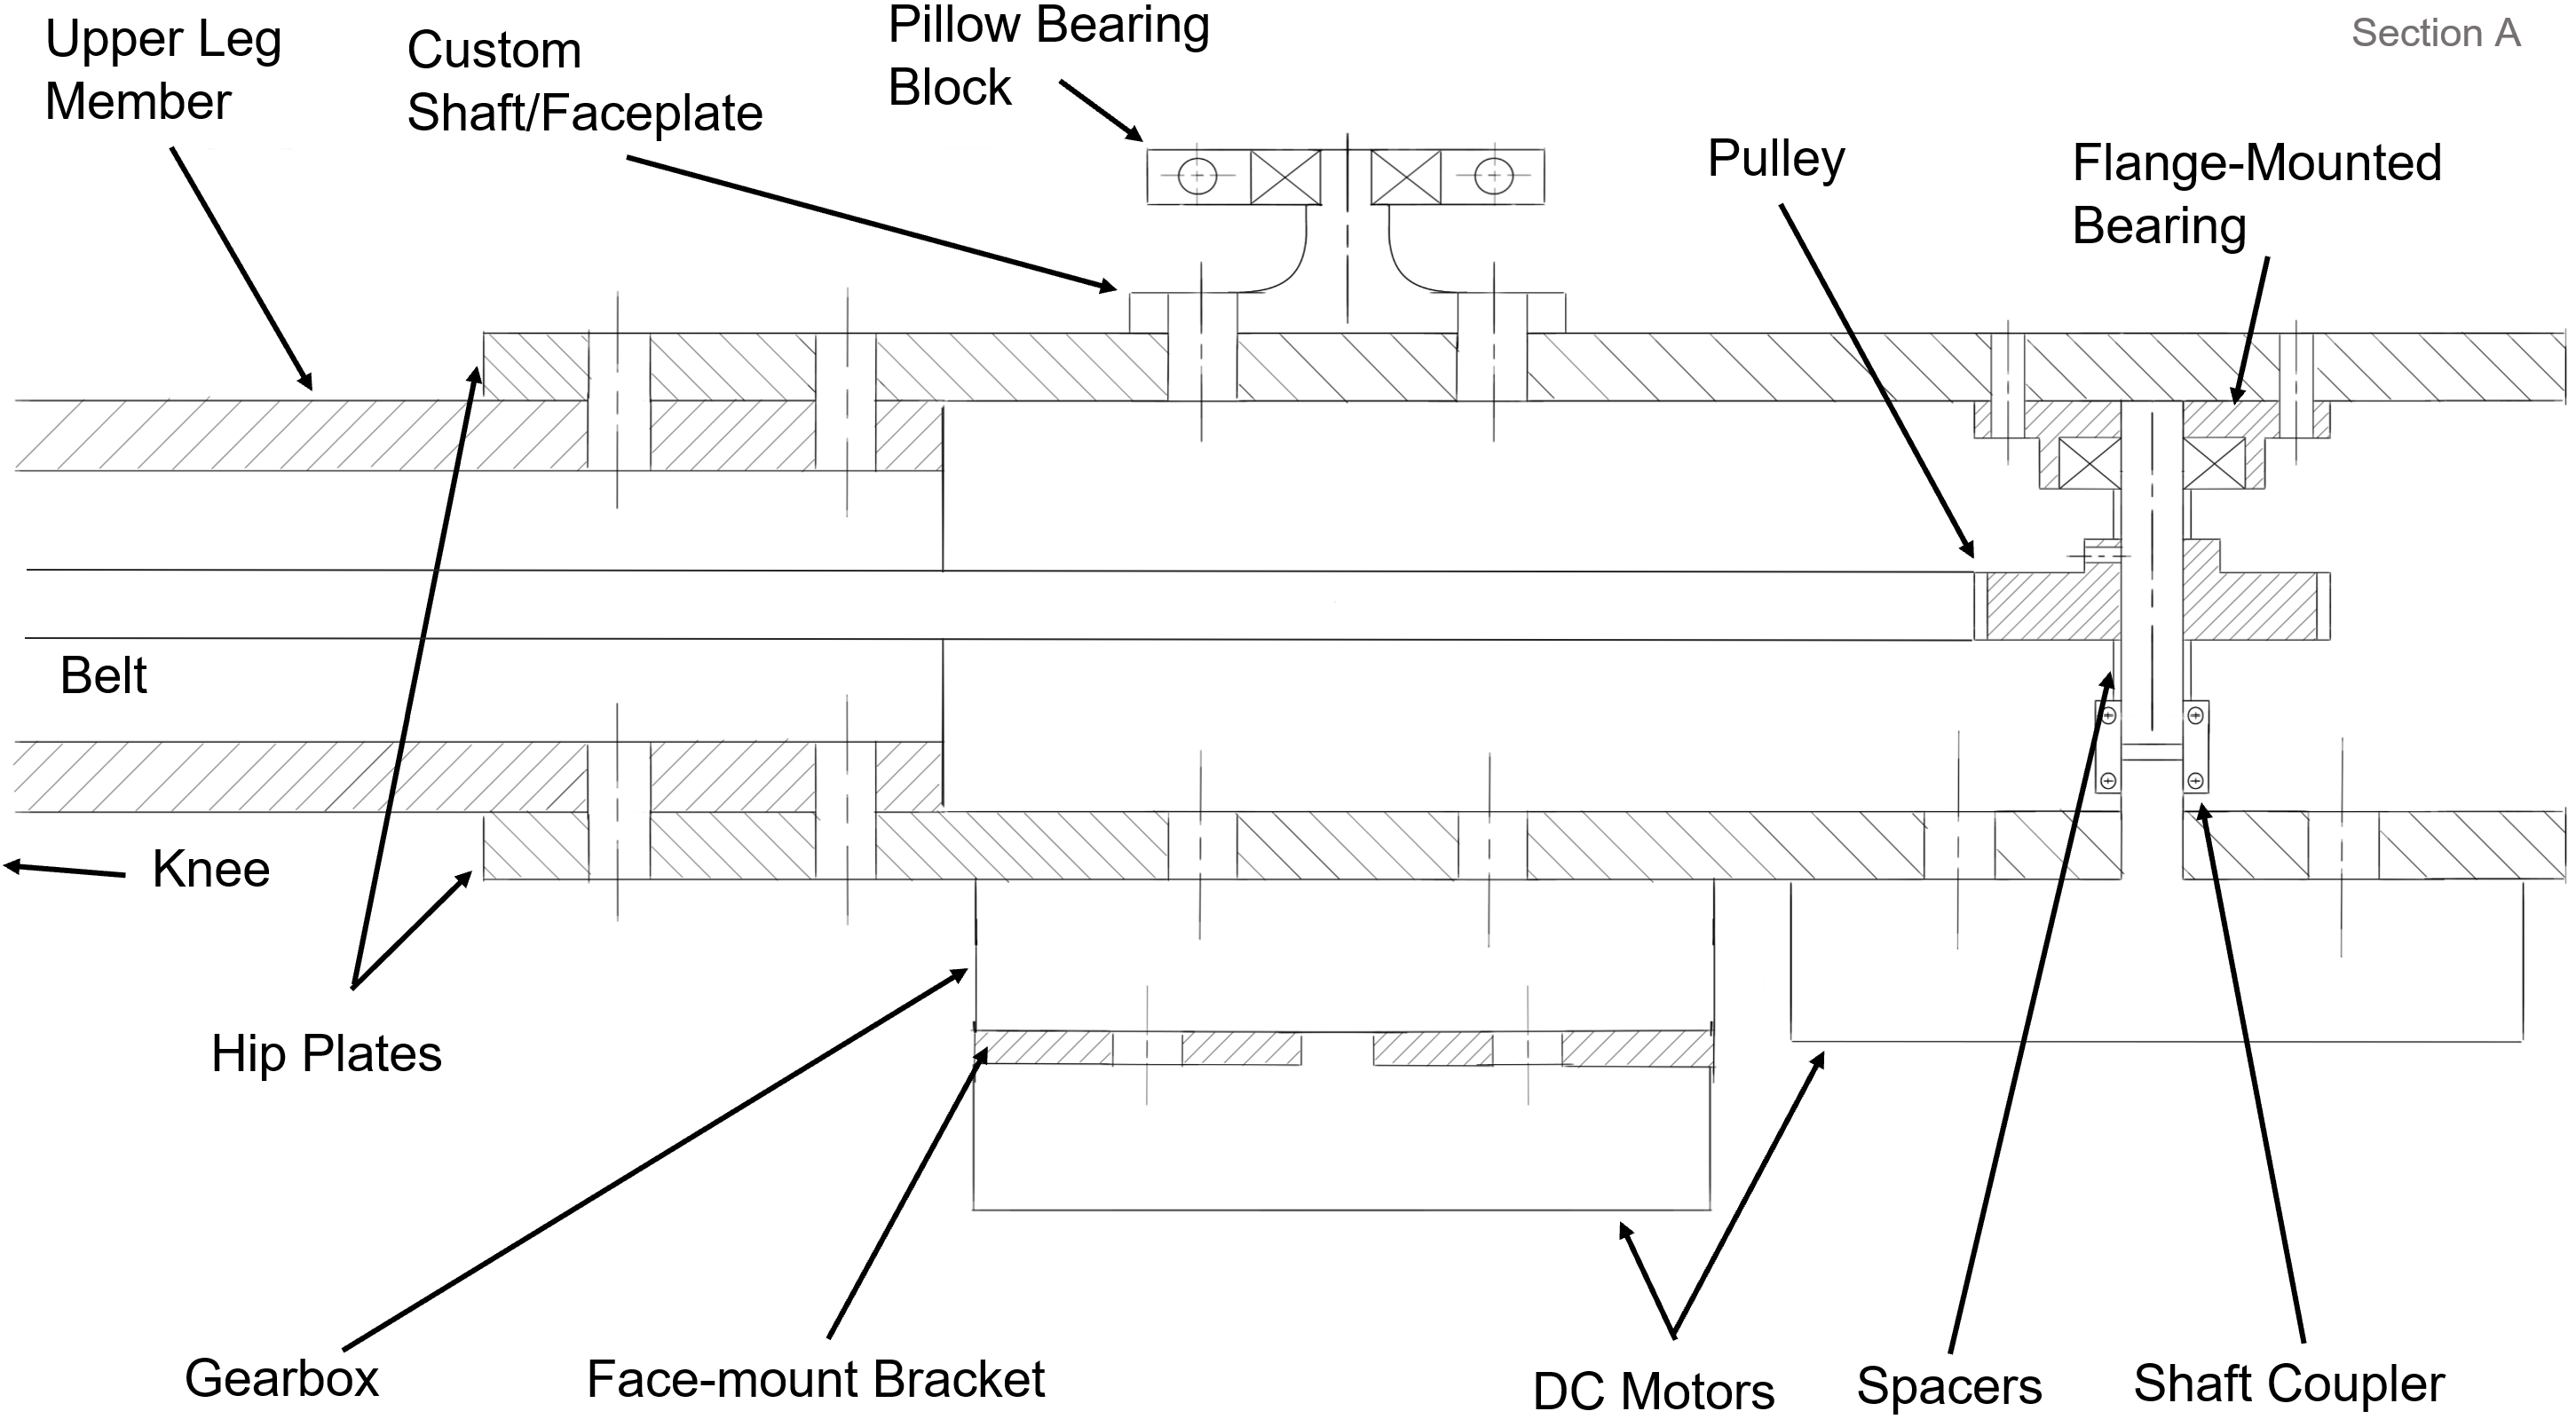
\includegraphics[width=\textwidth]{2_DesignSolution/img/crab_hip.png}
    \caption{Crab Hip Top View}
    \label{fig:crab_hip}
\end{figure}

\begin{figure}
    \centering
    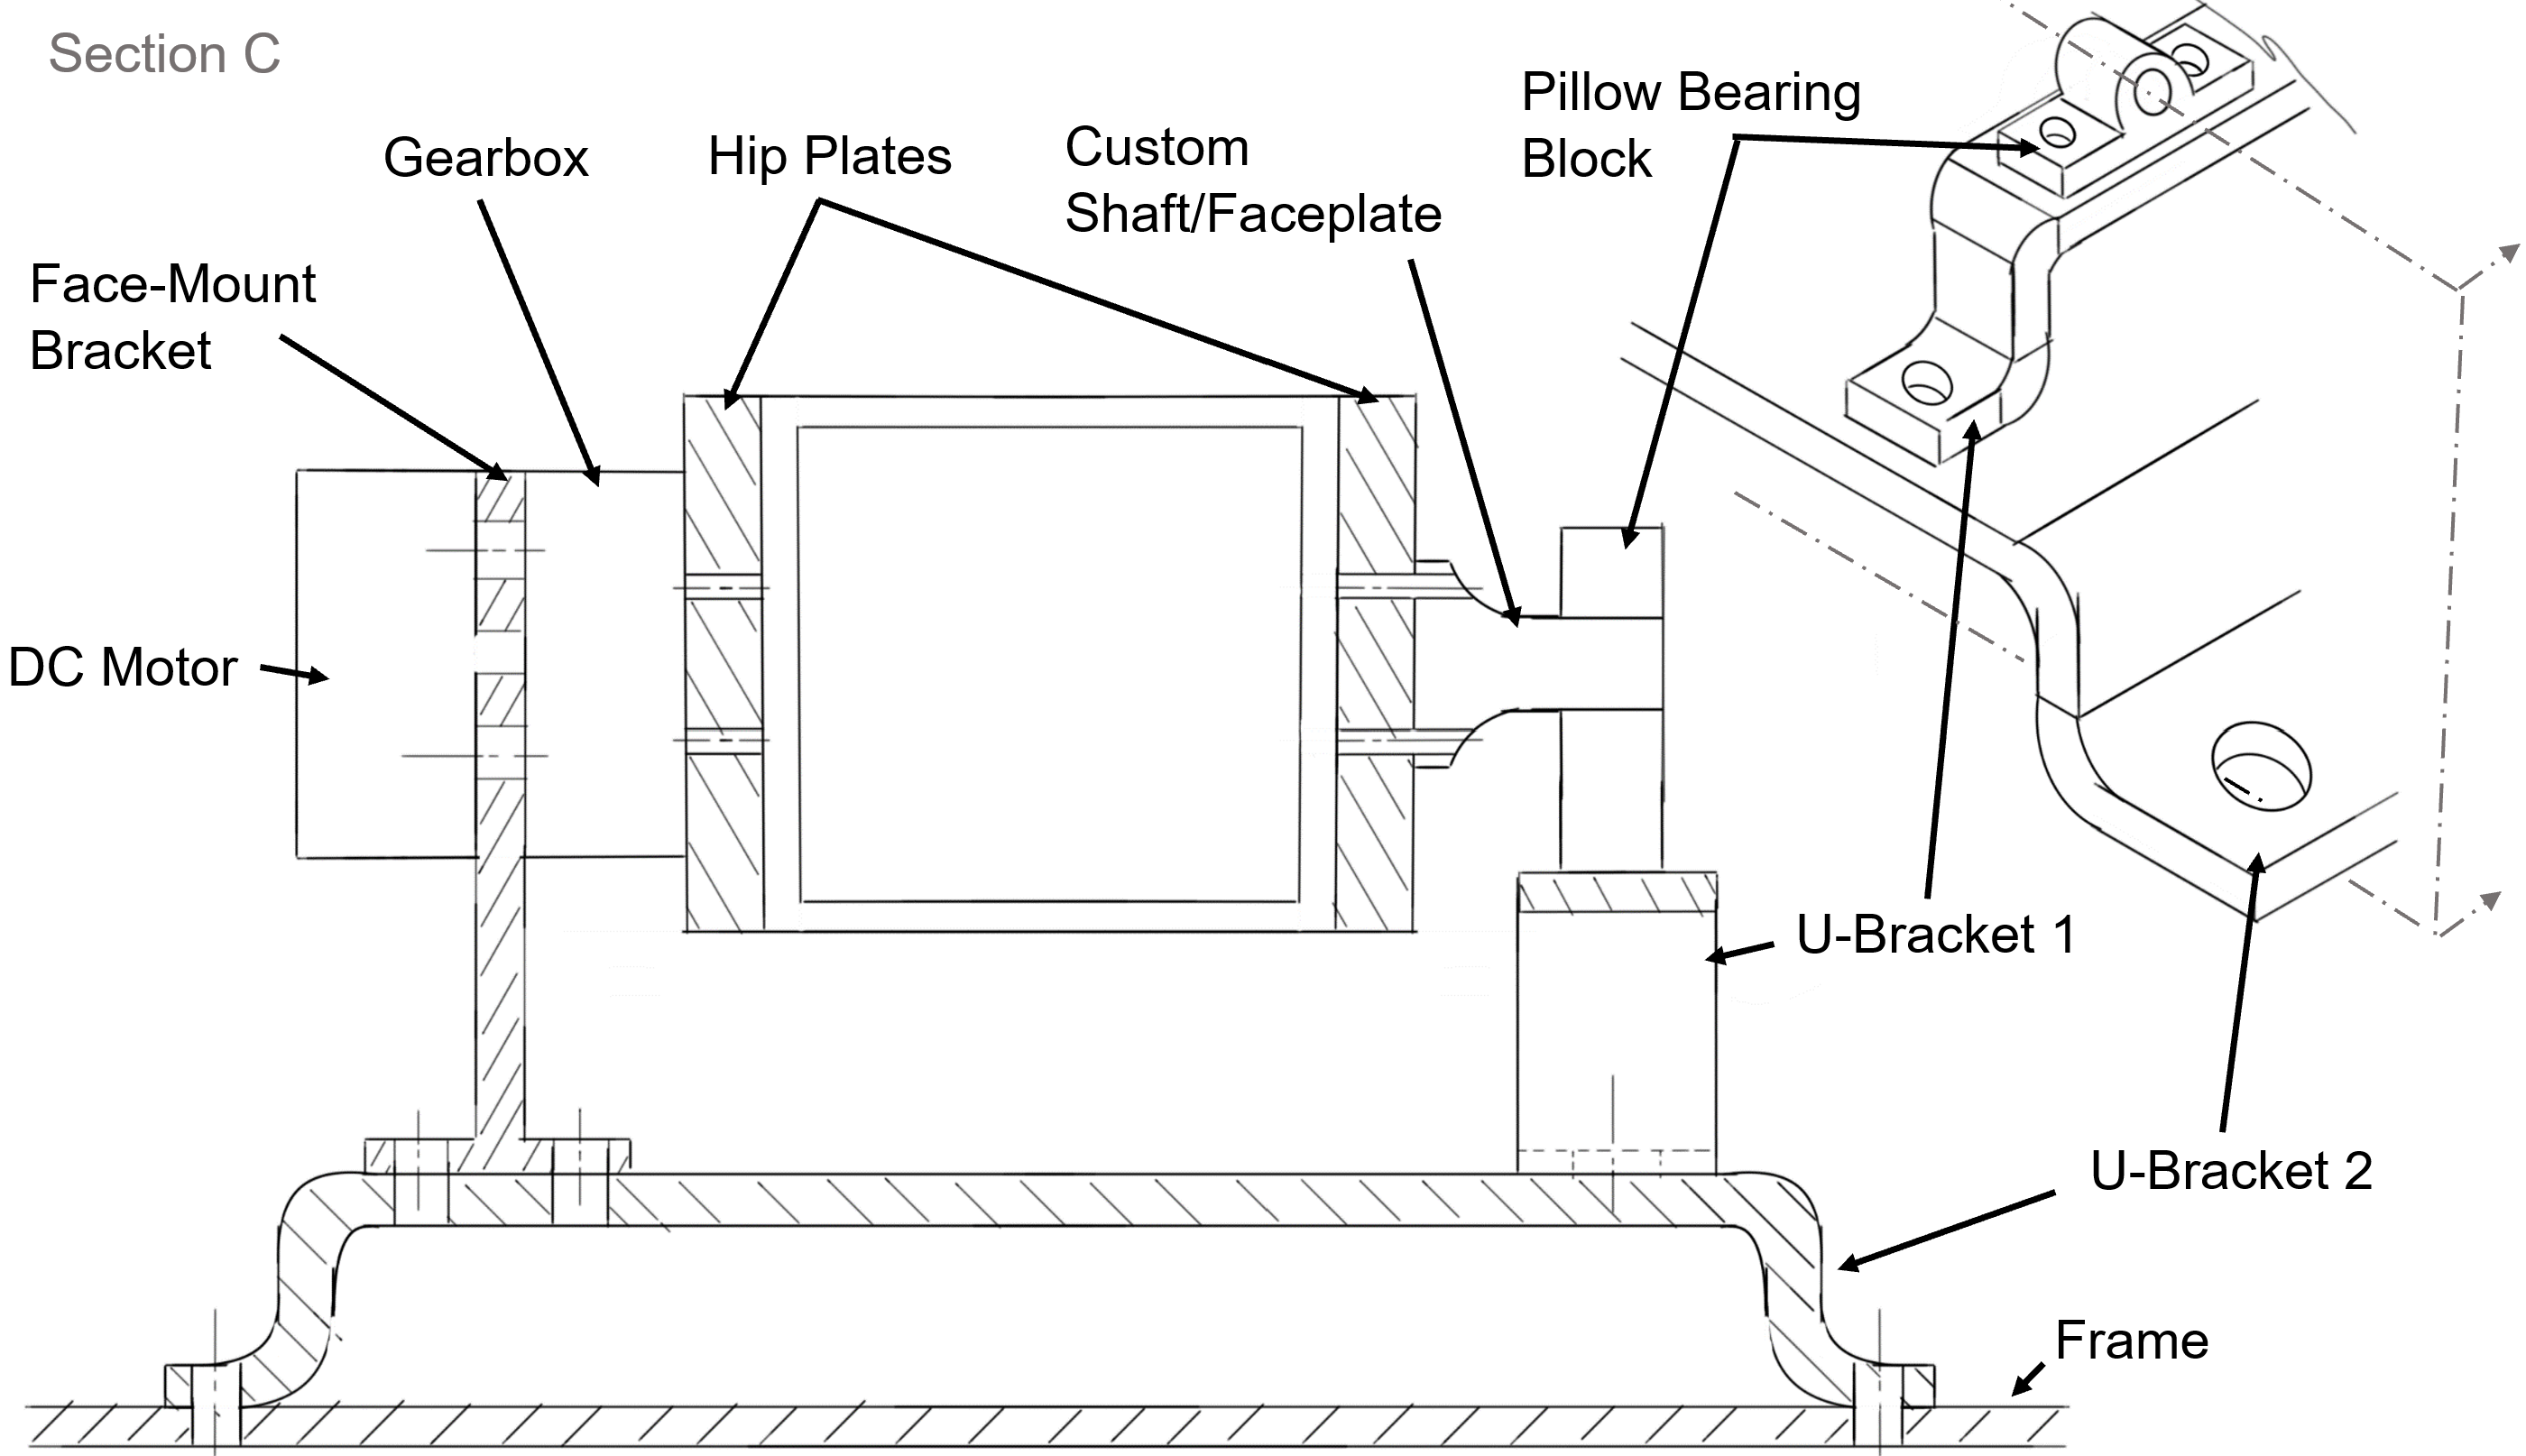
\includegraphics[width=\textwidth]{2_DesignSolution/img/crab_hip_cut.png}
    \caption{Crab Hip Section View}
    \label{fig:crab_hip_section}
\end{figure}